\newcounter{goals_counter}
\setcounter{goals_counter}{1}
\subsection{The Problem}
\begin{flushleft}
%%%%%%%%%%%%%%%%%%%%%%%%%%%%%%%%%%%
%%%%%%%%%%% THE PROBLEM %%%%%%%%%%%
%%%%%%%%%%%%%%%%%%%%%%%%%%%%%%%%%%%
The world's food supply chain is threatened by climate change and an unsustainable rate of rising population. Since the Telangana region largely participates in the world's food economy, the Telangana government is interested in pursuing initiatives aimed at mitigating the effect these issues. In this case, the Telangana government wants to reform the way they build their policies regarding food production. Their goal is to utilize digital public goods and community-centric approaches in order to build resiliency against these dynamic challenges by building policies that are more agile and data-driven. 
\smallskip\\
%%%%%%%%%%%%%%%%%%%%%%%%%%%%%%%%%%%
%%%%%% THE PROPOSED SOLUTION %%%%%%
%%%%%%%%%%%%%%%%%%%%%%%%%%%%%%%%%%%
This initiative, named {\bf D}ata-d{\bf R}iven Pr{\bf E}dictive F{\bf A}r{\bf M}ing, or DREAM, intends to provide a solution that focuses on serving the needs of three stakeholders: farmers, agronomists, and policy makers. DREAM will serve as a central tool for policy makers to access data about the region. For farmers, DREAM will serve as a tool to help them organize their own production data as well as provide an interface to seek for support from their community. Finally, agronomists will use DREAM as a tool to manage their work such as planning field visits or verifying the data provided by farmers. %% add more content here? more high level description of DREAM...

%%%%%%%%%%%%%%%%%%%%%%%%%%%%%%%%%%%
%%%%%%%%% GENERAL DIAGRAM %%%%%%%%%
%%%%%%%%%%%%%%%%%%%%%%%%%%%%%%%%%%%
\begin{center}
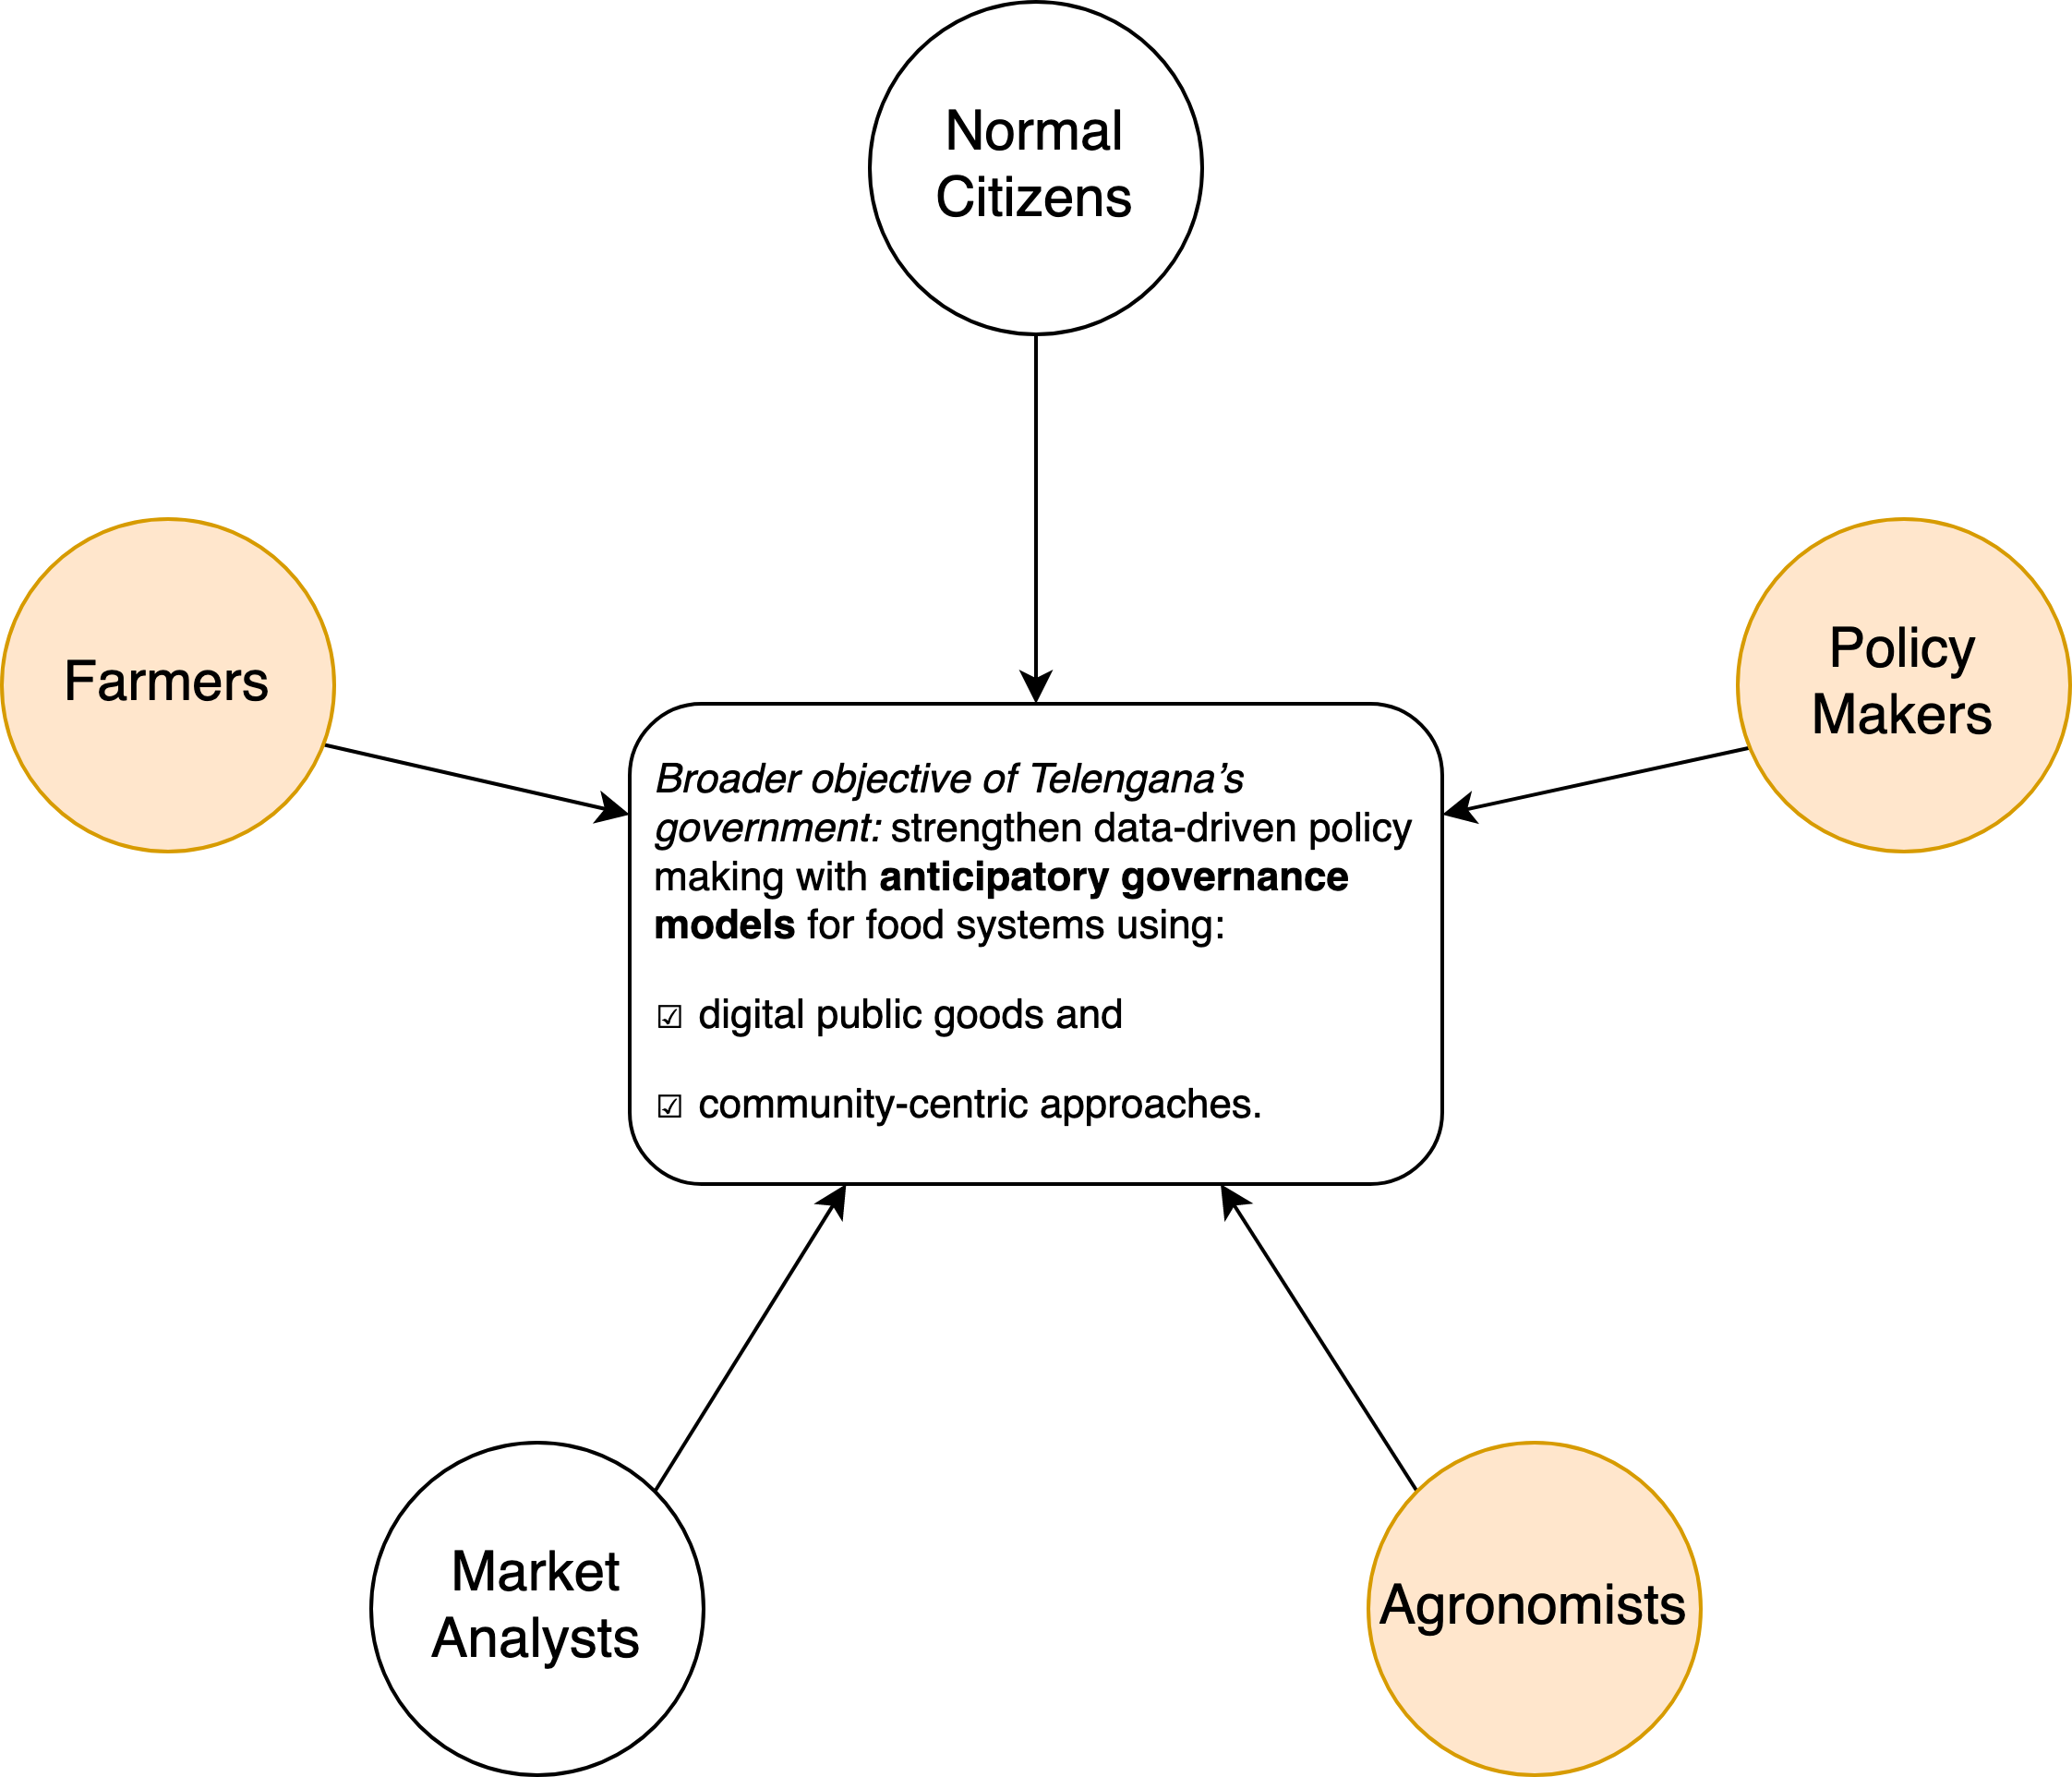
\includegraphics[scale=0.6]{../images_diagrams/stakeholders_in_broader_gov_objective.png}
\end{center}

%%%%%%%%%%%%%%%%%%%%%%%%%%%%%%%%%%%
%%%%%%%%% PURPOSE OF DOC %%%%%%%%%%
%%%%%%%%%%%%%%%%%%%%%%%%%%%%%%%%%%%
\subsection{General Purpose}
The purpose of this document is to provide a detailed description of the purposed software for the DREAM initiative. This includes the goals of the system, the phenomena related to the product, the functions of the product, the requirements related to the different interfaces, scenarios of using the product, and other details about the proposed system.
%\smallskip\\
\end{flushleft}

%%%%%%%%%%%%%%%%%%%%%%%%%%%%%%%%%%%
%%%%%%%%%%%% THE GOALS %%%%%%%%%%%%
%%%%%%%%%%%%%%%%%%%%%%%%%%%%%%%%%%%
\subsubsection{Goals}

The following table lists an aggregate collection of the goals that serve the three main stakeholders that are in the scope of this system.

%%%% GOALS TABLE %%%%
\begin{center}
\renewcommand{\arraystretch}{1.25}
\begin{tabular}{|c| >{\raggedright\arraybackslash}p{12cm}|} \hline
    \textbf{ID} & \textbf{Goals}\\
    \hline
    G\addOne{goals_counter}  & Farmers can visualize relevant data and suggestions based on their location and type of production.\\ 
    \hline
    G\addOne{goals_counter}  & Agronomists and farmers can view weather forecast data.\\ 
    \hline
    G\addOne{goals_counter}  & Farmers can interact with others farmers and agronomists by requesting for help and suggestions.\\
    \hline
    G\addOne{goals_counter}  & Farmers can create discussion forums with other farmers.\\
    \hline
    G\addOne{goals_counter}  & Agronomists can supervise a sub-area inside the region. \\
    \hline
    G\addOne{goals_counter}  & Agronomists can visualize the performance of the farmers in their sub-area.\\ %view the ranking of farmers’ performance in their specific area.
    \hline
    G\addOne{goals_counter}  & Agronomists can visualize and update a daily plan to visit farms in their area.\\
    \hline
    G\addOne{goals_counter}  & Agronomists can specify the deviations from their daily plan and confirm the execution of their daily plan at the end of each day.\\
    \hline
    G\addOne{goals_counter}  & Telengana’s policy makers can view the performance of the farmers and the ranking of the farmers.\\
    \hline
    G\addOne{goals_counter} & Telengana’s policy makers can determine if support from agronomists and well-performing farmers produces significant results.\\
    \hline
\end{tabular}
\end{center}

%%%%%%%%%%%%%%%%%%%%%%%%%%%%%%%%%%%
%%%%%%%%%%%%% PHENOMENA %%%%%%%%%%%
%%%%%%%%%%%%%%%%%%%%%%%%%%%%%%%%%%%
\subsection{Scope}

\begin{flushleft} %Here we include an analysis of the world and of the shared phenomena 
The scope of this document is to provide a comprehensive analysis of the requirements and specifications of the DREAM product. 
Considering the three users in the scope of this initiative, the design of the system must first consider the following phenomena in the context in which the system will operate.

%%%% PHENOMENA TABLE %%%%

\begin{table}[H]
\centering
\begin{tabular}{|p{0.55\textwidth}| c| c|}
\hline
\textbf{Phenomena}        & \textbf{Shared} & \textbf{Who controls it} \\ \hline

An agronomist visits a farm & N & W \\ \hline
Farmer has an issue with the farm & N & W \\ \hline
An agronomist confirms a plan and send all the data about the visits he performed  & Y & W \\ \hline
A farmer sends a message to an agronomist & Y &  W\\ \hline
A farmer creates a forum discussion & Y & W  \\ \hline
An agronomist responds to a farmer help or suggestion request & Y & W \\ \hline 
A user inspects data & Y & W \\ \hline
Policy maker flags poor performing and well performing farmers & Y & W \\ \hline

Data analysis is performed & N & M  \\ \hline
Statistics are created based on data analyzed  & N & M  \\ \hline
The system computes the best path connecting all farmers an agronomist has to visit  & N & M  \\ \hline
The system recommend farmers to be visited by an agronomist & N & M  \\ \hline
\end{tabular}

\caption{World and Machine Phenomena table}
\label{PhenomenaTable}
\end{table}

\end{flushleft}

\subsection{Definitions, Acronyms, Abbreviations}

%%%% DEFINITIONS TABLE %%%%

\begin{center}
\renewcommand{\arraystretch}{1.25}
\begin{tabular}{l >{\raggedright\arraybackslash}p{12cm} } \hline
    \textbf{Term} & \textbf{Definition}\\ 
    DREAM & The system described in this document; Data-dRiven PrEdictive FArMing\\
    User & Farmer, agronomist, or policy user; anyone who uses the system.\\

	Policy Maker & Member of the Telangana government who deploys and manages different agriculture-related policies. \\
	Agronomist & Professional who specializes in agriculture sciences. \\
    Farmer & A user who uses DREAM to help manage data relating to their farms and fields.\\
    Field & One enclosed area that corresponds to one crop. Many fields can make up a farm. The locations of the various fields do not need to be co-located.\\
    Farm & A set of one or many fields that are managed by one farmer.\\
    Production yields & The amount of crop harvested compared to the amount of crop planted. Measured comparatively by percentage or numerically by weight.\\
    Flag & A marker on a farmer that signals the system to increase the priority for the farmer to get visited by an agronomist.\\
    \hline
\end{tabular}
\end{center}

\subsection{Revision History}
\subsection{Reference Documents}
\subsection{Document Structure}